The extension of the material point method to the DG approximation has been motivated in the previous section and is developed hereinafter. After a brief historical review of DG methods, the Discontinuous Galerkin Material Point Method (DGMPM) is derived within the large strain framework with a total Lagrangian formulation. It will then be seen that this new numerical approach uses the approximate-state Riemann solver developed in section \ref{sec:riemann_solvers} to compute terms at elements interfaces which purpose is to connect elements together. At last, the DGMPM solution scheme will be provided for hyperbolic problems.

\subsection{The discontinuous Galerkin approximation}
The DG approximation was first introduced in the context of the finite element method for the solution of the neutron transport equation \cite{NeutronDG}. This hyperbolic equation describes the advection of the angular flux which quantifies the amount of neutrons at a given location. Since neutrons can lie in a cell of a finite element mesh while its neighbors are empty, the need of describing discontinuities of the primal field across elements interfaces within a FEM context arised. Hence, an approximate solution was seeked by the Galerkin method, in a domain discretized with triangular elements by means of Lagrange polynomials that can be discontinuous across the cells. This approach amounts to duplicate the nodes of the mesh so that the support of each shape function reduces to one finite element. Those early works have launched a series of developed of the Discontinuous Galerkin Finite Element Method (DGFEM) for parabolic \cite{Arnold_IPM}, elliptic \cite{Hansbo_DGsolid,Noel_HEDG}, and hyperbolic problems \cite{Cockburn}. Indeed, the DGFEM gained more and more popularity since the 80's due to its ability to locally handle high-order approximation and its highly parallelizable nature. 
%However, the increase of the dimension of the discrete it implies led more recently to the formulation of Hibridizable Discontinuous Galerkin methods (HDG) \cite{Cockburn_HDG0,Cockburn_HDG1,Cockburn_HDG2}.
For application to hyperbolic problems, of particular interest here, researches enabled the introduction of numerical tools developed for Finite Volume Methods (FVM) within finite element schemes. Namely, the use of suitable \textit{slope limiters} \cite{vanLeer_Limiters} based on the \textit{total variation} \cite{Harten_TVD} allowed the formulation of flexible numerical methods in which high resolution of discontinuities, without destroying the accuracy in smooth regions, is possible. Furthermore, this approach can easily handle mesh-adaption strategies due to the relaxation of fields continuity. Nevertheles the mesh tangling problems do not vanish.

An extension of PIC to DG approximation for the solution of Maxwell's equations is proposed in \cite{DGPIC_maxwell} and \cite{Stindl_DGPIC} in which different projections of fields between the grid and particles are used. Although those methods allow local high-order approximation, particles do not carry all th fields and the DGPIC, as the original PIC, cannot be considered as a fully Lagrangian approach.

Considering the prior discussion, the development of the DGMPM may lead to a numerical method that benefits from both FEM and FVM features, enables local high-order approximation and avoids mesh entanglement instabilities. 


% %%%%%%%%%%%%%%%%%%%%%%%%%%%%%%%%%%%%%%%%%%%%%%%%%%%%%%%%%%%%%
% % Hyperbolic
% The \textit{discontinuous Galerkin (DG)} approximation enables to build numerical schemes that benefit from both finite element and finite volume methods. 
% Parler des limiteurs \cite{vanLeer_Limiters} pour atteindre la notion de schéma TVB et TVDM (TVD \cite{Harten_TVD}). Extension to RK so that the scheme can reach locally high order accuracy. In addition, the same order of accuracy is reached for velocity and gradients within a finite element framework when the weak form is based on a conservation laws system. 

% % In parallel, for parabolic or elliptic
% \cite[parabolic+penalties]{Arnold_IPM},\cite{Hansbo_DGsolid},\cite[elliptic]{Noel_HEDG}: Three field Hu-Washizu variational formulation ; assumed form of deformation gradient ; Total Lagrangian ; penalization of displacement jumps; Advantages--Drawbacks in note books

% % Introduction of HDG
% \cite{Cockburn_HDG0},\cite{Cockburn_HDG1},\cite{Cockburn_HDG2}: HDG for elliptic problems (differrence between LDG-H and HDG ?)

% % Recently extended to hyperbolic problems in solid dynamics
% \cite{NGuyen_HDG} for application to solid mechanics and extension to hyperbolic problems. Solved for displacement with enforced continuity across elements interfaces. Does not use the characteristic structure as what is done in finite volumes or original DGFEM

% However, all those approaches based on the primal field do not use the characterisitc structure. Dans l'état, ça ne peut pas être appliqué à la méca des solides puisque l'on est obligé d'imposer la continuité du champ de déplacement et donc de formuler le problème en u.
% \begin{itemize}
% \item \cite{Chavent_Salzano,Chavent_Cockburn,Cockburn_Shu,DGFEM_CFL,Cockburn}:
% \item \cite{Chavent_Salzano}--\cite{Cockburn} developments of DGFEM (mainly for fluid mechanics ?)
% \item \cite[parabolic+penalties]{Arnold_IPM},\cite{Hansbo_DGsolid},\cite[elliptic]{Noel_HEDG}: Three field Hu-Washizu variational formulation ; assumed form of deformation gradient ; Total Lagrangian ; penalization of displacement jumps; Advantages--Drawbacks in note books
% \item \cite{Cockburn_HDG0},\cite{Cockburn_HDG1},\cite{Cockburn_HDG2}: HDG for elliptic problems (differrence between LDG-H and HDG ?)
% \item \cite{NGuyen_HDG} for application to solid mechanics and extension to hyperbolic problems. Solved for displacement with enforced continuity across elements interfaces. Does not use the characteristic structure as what is done in finite volumes or original DGFEM
% \item \cite{DGPIC,DGPIC_maxwell}: application to PIC
% \end{itemize}


% RKDG - limiters - TVD - CFL - HDG (steady convection-diffusion problem (elliptic problem)) - HE DG
% Applied to steady solid mechanics problems for the ability of local high order approximation ?
% Continuity of displacement enforced through Lagrange multipliers. Benefits from superconvergence properties. A priori on utilise plus du HDG en méca du solide \cite[ALE]{NGuyen_HDG} + postprocessing pour le champ de déplacement + implicit en dynamique. Originally developed in \cite{Cockburn_HDG0}: "we may define more generally as a hybrid method any finite element method based on a formulation where one unknown is a function, or some of its derivatives, on the set $\Omega$, and the other unknown is the trace of some of its derivatives of the same function, or the trace of the function itself, along the boundaries of the set K". Numerical traces \cite{Cockburn_HDG1}


\subsection{The DGMPM discretization}
As for MPM, a continuum body $\Omega_t$ is discretized within the time interval $\tau$ into a set of $N_p$ material points in an arbitrary Cartesian grid made of  $N_n$ nodes and $E$ non-overlapping cells of volume $\Omega^e$. The boundary of the domain is defined, as in section \ref{sec:MPM} (see the two-dimensional example in figure \ref{fig:domain}), by boundary particles.

Since the DGMPM is expected to provide a material description of a deformation, we seek an approximate solution of a Lagrangian system of conservation laws written in conservative form, by means of a weak form. Recall that such a conservative form for some vecotr of conserved quantities $\Wcb$ reads, in Cartesian coordinates system:
%The DGMPM is also based on a weak formulation. Indeed, we seek an approximate solution of a Lagrangian system of conservation laws written in conservative form with a Cartesian coordinates system:
\begin{equation}
  \label{eq:conservative_form}
  \drond{\Wcb}{t} + \sum_{\alpha=1}^D \drond{\Fcb\cdot \vect{e}_\alpha}{X_\alpha} = \Scb \quad \forall \vect{X},t \in \Omega_0 \times \tau
\end{equation}
The key idea of DG methods is to allow jump of fields across mesh elements faces by using broken polynomials spaces \cite[Sec.~1.2.4]{DiPietro}:
\begin{equation}
\Vscr^k = \{ \Vcb \in H^k\Omega^e) \} \quad ;\quad \Vscr_h^k = \{\Vcb \in \Pscr^k(\Omega^e) \} \subset \Vscr^k
\end{equation}
with $H^k(\Omega^e)$, the Sobolev space and $\Pscr^k(\Omega^e)$, the space of polynomials of degree $k$ in $\Omega^e$. We restrict our attention here to linear polynomials, that is $k=1$. Those broken polynomials spaces yield a weak form of equation \eqref{eq:conservative_form} written element-wise. After integration by part, one gets:
\begin{equation}
  \label{eq:DGMPM_weak_form}
  \begin{aligned}
    &\text{Find $\Wcb \in \Vscr_h^1$ such that} \\
    &\int_{\Omega^e} \drond{\Wcb}{t} \vect{\Vc} \: d\Omega - \int_{\Omega^e} \Fcb_\alpha  \drond{\vect{\Vc}}{X_\alpha} \: d\Omega   + \int_{\partial \Omega^e} \(\Fcb\cdot \vect{N}\)  \vect{\Vc} \: d\Gamma = \int_{\Omega^e} \Scb \vect{\Vc} \: d\Omega \quad \forall \: \vect{\Vc},e,t \in  \Vscr_h^1\times \[1,E\]\times \tau
  \end{aligned}
\end{equation}
where $\partial \Omega^e$ is the boundary of the $e$th element with outward normal vector $\vect{N}$. The intercell flux is writtten $\Fcb_N$ for simplicity. 
%Those numerical fluxes can be computed from the solution of an approximate Riemann solver \cite{Trangenstein} (see section \ref{}). In particular, the stationary solution of Riemann problems defined at element boundaries $\Gamma_i$ such that $\cup_i \Gamma_i = \Gamma_e $  gives the well-known \textit{Godunov's method}.
The introduction of the delta Dirac characteristic function for material points density, combined to the writing of specific quantities:
\begin{align}
& \rho_0\(\vect{X}\) =  \sum_{p=1}^{N_p} m_p \delta\(\vect{X}^p - \vect{X}\) \\
& \Wcb = \rho_0 \bar{\Wcb} \quad ; \quad \Fcb_\alpha = \rho_0 \bar{\Fcb}_\alpha \quad ; \quad \Scb = \rho_0 \bar{\Scb}
\end{align}
leads to the following weak form of the total Lagrangian formulation:
%Such a discretization of the reference mass density combined with the writing of Lagrangian conservation laws \eqref{eq:conservative_form} yields a total Lagrangian formulation, and equation \eqref{eq:DGMPM_weak_form} thus reads:
\begin{equation} 
  \label{eq:DGMPM_discrete_weak}
  \sum_{p=1}^{N_p} m_p\[\drond{\bar{\Wcb}}{t}  \vect{\Vc} - \bar{\Fcb}_{\alpha} \drond{\vect{\Vc}}{X_\alpha} -\bar{\Scb}  \vect{\Vc} \]_{|\vect{X}=\vect{X}^p} + \int_{\partial \Omega^e} \Fcb_N  \vect{\Vc} \: d\Gamma = 0 \quad \forall \: \vect{\Vc},e,t \in  \Vscr_h^1\times \[1,E\]\times \tau
\end{equation}

Material points are viewed as interpolation points so that the fields of the weak form \eqref{eq:DGMPM_discrete_weak} are evaluated from nodal values with the shape functions $S(\vect{X})$:
\begin{equation}
  \label{eq:DGMPM_node2points}
  \bar{\Wcb}(\vect{X}^p) = \bar{\Wcb}^p =\sum^{N_n}_{i=1} S_{i}(\vect{X}^p)\bar{\Wcb}^i = \sum^{N_n}_{i=1} S_{ip}\bar{\Wcb}^i 
\end{equation}
$\bar{\Wcb}^i$ hence denotes the specific vector of conserved quantities at node $i$. In the following, the same convention than before, consisting in denoting particles values by index $p$ and nodal ones by $i$ or $j$, is used. 

Combination of equations \eqref{eq:DGMPM_discrete_weak}-\eqref{eq:DGMPM_node2points} and arbitrariness of the test field yield the semi-discrete system that must be solved on the grid:
\begin{equation}
  \label{eq:DGMPM_semi_discrete}
  \sum_{p=1}^{N_p}\[ S_{ip} m_p S_{jp} \drond{\bar{\Wcb}^j}{t}  - \drond{S_{ip}}{X_\alpha} m_p S_{jp} \bar{\Fcb}^j_{\alpha} - S_{ip} m_p \bar{\Scb}^p\] + \int_{\Gamma_e} S_i(\vect{X}) \Fcb_N  \: d\Gamma =  0  \quad \forall \: e,t \in  \times \[1,E\]\times \tau
\end{equation}
or, in matrix form:
\begin{equation}
  \label{eq:DGMPM_semi_discrete_matrix}
   M_{ij} \drond{\bar{\Wcb}_j}{t} - K^\alpha_{ij} \bar{\Fcb}^j_{\alpha} - \Scb^i + \vect{\hat{\Fc}}^i = \vect{0}  
\end{equation}
Note that the consistent mass matrix $M_{ij}$ may also be singular when only one material point lies in an element due to reduced integration. Hence, the diagonally lumped mass matrix $M^L_i$ is used.
%% remark environment for the above remark
% \begin{remark}
% The consistent mass matrix $M_{ij}$ may also be singular when only one material point lies in an element due to reduced integration. Hence, the diagonally lumped mass matrix $M^L_i$ is used. 
% \end{remark}

%% Expression of matrices
% In system \eqref{eq:DGMPM_semi_discrete_matrix}, the consistent mass matrix and the \textit{pseudo-stiffness} matrix are respectively defined as:
% \begin{subequations}
%   \begin{alignat}{1}
%     \label{eq:DGMPM_mass_matrix}
%     & M_{ij}= \sum_{p=1}^{N_p} m_p  S_{jp} S_{ip} \\
%     \label{eq:DGMPM_pseudo-stiffness}
%     & K^\alpha_{ij} = \sum_{p=1}^{N_p} m_p\drond{S_{ip}}{X_\alpha} S_{jp} \bar{\Fcb}_{\alpha,j}
%   \end{alignat}
% \end{subequations}


Finally, the explicit forward Euler time discretization of $\tau$ in $N_t$ subinterval is perfomed, leading to the discrete system:
\begin{equation}
  \label{eq:DGMPM_discrete}
  M^L_i \frac{\bar{\Wcb}^{i,n+1} - \bar{\Wcb}^{i,n}}{\Delta t^{n} } = K^\alpha_{ij} \bar{\Fcb}_{\alpha}^{j,n} + \Scb^{i,n}- \vect{\hat{\Fc}}^{i,n}  
\end{equation}
where again, the superscripts $\bullet^{k,l}$ denote a field evaluated at node $k$ and time step $l$.
Alternatively, a \textit{second-order Runge-Kutta (RK2)} explicit time discretization may be used, leading to the following two-stages discrete form:
\begin{align}
  \label{eq:DGMPM_discrete_RK2}
  & M^L_i \frac{\bar{\Wcb}^{i,n+1/2} - \bar{\Wcb}^{i,n}}{\Delta t^{n} } = \frac{1}{2}\(K^\alpha_{ij} \bar{\Fcb}_{\alpha}^{j,n} + \Scb^{i,n}- \vect{\hat{\Fc}}^{i,n}\)  \\
  & M^L_i \frac{\bar{\Wcb}^{i,n+1} - \bar{\Wcb}^{i,n}}{\Delta t^{n} } = K^\alpha_{ij} \bar{\Fcb}_{\alpha}^{j,n+1/2} + \Scb^{i,n+1/2}- \vect{\hat{\Fc}}^{i,n+1/2}
\end{align}
\begin{remark}
  We chose here one possible two-stages second order Runge-Kutta method among others. See for instance \cite[Sec.~10.4.2]{Leveque} for a Total Variation Diminishing version of the RK2 time discretization. 
\end{remark}

Note that in general the source term $\Scb$ in equation \eqref{eq:conservative_form} may depend on the vector of conserved quantities, hence the superscript $n$ in equations \eqref{eq:DGMPM_discrete} and \eqref{eq:DGMPM_discrete_RK2}. 
%The computation of interface fluxes $\hat{\Fcb}^i$ is now developed.

\subsection{Non-homogeneous hyperbolic system}
%\subsubsection{Non-homogeneous hyperbolic system}
Solid mechanics equations may lead to source terms in the conservative form even for neglected body forces. This is for instance the case for time-dependent plasticity (see $\Scb$ in equation \eqref{eq:vectors_elasticity}), or for cylindrical or spherical coordinates systems. In the latter siuationss, the gradient operators invlove not only derivatives leading to a right-hand side in system \eqref{eq:conservative_form} that depends on $\Wcb$ and called a geometric source term \cite[Ch.~17]{Leveque}. Efficient procedures for the treatment of source terms $\Scb$ in non-homogeneous hyperbolic systems have been developed for finite volume methods that we propose here to take advantage of. 

A commonly used approach to solve non-homogeneous systems consists in solving alternatively a homogeneous system and a system of ODEs, namely:
\begin{subequations}
  \begin{alignat}{1}
    \label{eq:Splitting_advec} 
    & \drond{\Wcb}{t} + \sum_{\alpha=1}^D \drond{\Fcb\cdot \vect{e}_\alpha}{X_\alpha} = \vect{0}\\
    \label{eq:Splitting_ODE}
    & \ddroit{\Wcb}{t} = \Scb
  \end{alignat}
\end{subequations}
Equation \eqref{eq:Splitting_advec} is solved by applying the DGMPM discretization \eqref{eq:DGMPM_discrete}, while the solution of equation \eqref{eq:Splitting_ODE} is determined by using well-known ODEs solvers. If we denote by $H^{(\Delta t)}$ and $F^{(\Delta t)}$ the discrete solution operators associated to equations \eqref{eq:Splitting_advec} and \eqref{eq:Splitting_ODE} respectively for one time step, the discrete solution reads \cite{Toro}:
\begin{equation}
  \label{eq:godunov_splitting}
  \Wcb^{n+1} = F^{(\Delta t)} H^{(\Delta t)} (\Wcb^n)
\end{equation}
Two sub-problems are thus solved separately at each time step, the solution of the first one being used as initial conditions for the second one. Hence, \textit{Fractional-step} or \textit{Splitting} methods enable to taking advantage of efficient tools already developed both for homogeneous systems of conservation laws and for ODEs. 

\begin{remark}
  The fractional-step method \eqref{eq:godunov_splitting}, known as Godunov's splitting, is only first–order accurate in time, when S and C are at least first–order accurate solution operators. On the other hand, Strang splitting:
  \begin{equation}
    \label{eq:Strang_splitting}
    \Wcb^{n+1} = F^{(\Delta t/2)} H^{(\Delta t)} F^{(\Delta t/2)} (\Wcb^n)
  \end{equation}
is second-order accurate if each solution operator is at least second-order accurate \cite{Leveque}.
\end{remark}
%\cite[p.548]{Toro}, \cite{Thomas_EVP}

Note that the DGMPM solution scheme reduces to the discrete solution oparator $H^{(\Delta t)}$, or $H$ for simplicity, which in turn, aims at find approximate similarity solutions since it only solves homogeneous systems (recall remark \ref{rq:similarity_solution} in section \ref{sec:characteristic_analysis}). For a DGMPM space-time discretization made of $N_p$ material points and $N_T$ time increments, those solutions can be written:
% It has been established so far that the DGMPM scheme provides an approximate solution $\Qc(\vect{X}^i,t^{n,+1})= \Qc^{i,n+1}$,  with $i=1,...,N_n$ and $n=1,...,N_T$, that depends on the value of $\Qc$ at other points and previous time step, that is:
\begin{equation}
  \label{eq:general_scheme}
  \Qc^{i,n+1}= H \(\Qc^{j,n}\) \quad j=1...,N_n \: ; \: n=1,...,N_T
\end{equation}
where the set of nodes $j$ having an influence on $\Qc^i$ defines the \textit{stencil} of the method. 
\begin{definition}
  \label{def:monotonicity}
  A numerical scheme is said \textbf{monotone} if it satisfies:
  \begin{equation}
    \drond{H}{\Qc^j} \geq 0 \quad \forall j
  \end{equation}
\end{definition}
The following statement then holds:
\begin{theorem}[Godunov]
  \label{th:Godunov}
  Monotone linear numerical schemes can be at most first-order accurate.
\end{theorem}


\subsection{Interface fluxes}
\label{subsec:interface_fluxes}
DG methods for hyperbolic problems are based on the requirement of ensuring monotonicity of the scheme for piecewise constant approximation \cite{Cockburn}, namely, when the discrete system identifies with a finite volume one. Such a numerical method is monotone for flux functions $\Fcb_N$ that are Lipschitz continuous, consistent and monotone, namely, they must be \textit{E-fluxes} \cite{Osher}. One possibility, which is widely used and adopted here, is the \textit{Godunov flux function}. 
%The computation of interface fluxes $\hat{\Fcb}^{i,n}$ in the DGMPM system of discrete equations \eqref{eq:DGMPM_discrete} is now developed. We can here benefit from the finite volume technologies which are essentially based on the way those fluxes are computed.
\subsubsection*{The Godunov flux}
The Godunov method \cite{Godunov_method} has been proposed in the context of finite difference schemes in which the piecewise constant approximation of the solution naturally allowed the definition of local Riemann problems at cells interfaces. That is, two cells $i$ and $i+1$ with interface having normal vector $\vect{N}$ define a Riemann problem in the direction $X_N=\vect{X}\cdot{N}$, which \textit{stationary solution} is used to compute the intercell numerical flux $\Fcb \cdot \vect{N}$. The stationary solution, denoted by $\Wcb^*$, is the similarity solution along the vertical characteristic in the $(X_N,t)$ plane of the Riemann problem:
% Hence, the intercell numerical flux $\Fcb \cdot \vect{N}()$ is that of the stationary solution, that is, the similarity solution along the vertical straight line in the $(x,t)$ plane $\Wcb(x/t=0)$, of the Riemann problem:
\begin{equation}
  \label{eq:RP_mesh}
  \begin{aligned}
    &\drond{\Wcb}{t} + \drond{\Fcb_N}{X_N} = \vect{0}  \\
    & \Wcb(X_N,0)= \left\lbrace 
      \begin{aligned}
        & \Wcb_{X_N^-} \text{ if } X_N <0 \\
        & \Wcb_{X_N^{+}} \text{ if } X_N \geq 0
      \end{aligned}
        \right.
  \end{aligned}
\end{equation}
where $\Wcb_{X_N^-}$ and $\Wcb_{X_N^{+}}$ are the states lying infinitely close to the interface in cells $i$ and $i+1$. 
Godunov's method hence allows to account for the complete wave structure of the solution within the numerical scheme. Since this method is known to based on E-fluxes, intercell fluxes involved in boundary integrals of DG-methods weak forms are computed as Godunov's ones. To this end, Riemann problems are defined at cells faces by considering that initial data are piecewise constant even for high-order approximations. Note that this strategy is also followed in FVM when high-order reconstruction technics of the fields are used on the grid.

Let us consider as an illustration of the computation of interface fluxes within the DGMPM, the two-dimensional case depicted in figure \ref{fig:2D_edge}. Since intercell fluxes must be calculated in addition to the solution discrete equations \eqref{eq:DGMPM_discrete}, only one Riemann problem per interface is considered rather than nodal ones, in order to avoid a dramatical increase in computational time. Thus, by averaging the nodal values on each side of the interface, one obtains mean \textit{downwind} and \textit{upwind} states $\Wcb_{X_N^-}$ and $\Wcb_{X_N^+}$ that correspond to the initial conditions of the Riemann problem (see figure \ref{fig:2D_edge}).
\begin{figure}[h!]
  \centering
  \begin{tikzpicture}[scale=0.5]
  \draw (10.,0.) -- (12.,6.) ; 
  \draw[fill=black] (9.85,0.1) circle (0.1) node [left] {$1$};	
  \draw[fill=black] (10.2,-0.0) circle (0.1) node [right] {$2$};	
  \draw[fill=black] (11.85,6.1) circle (0.1) node [left] {$4$};	
  \draw[fill=black] (12.2,6) circle (0.1) node [right] {$3$};	
  \draw[->,very thick] (11.,3.) -- (12,3 -1/3) node [right,below] {$X_N$}; 
  \node at (8,3.5) {$\vect{\Qc}_{L} = \frac{\vect{\Qc}_1 + \vect{\Qc}_4}{2}$}; \node at (14.5,3.5) {$\vect{\Qc}_{R} = \frac{\vect{\Qc}_2 + \vect{\Qc}_3}{2}$};
\end{tikzpicture}

  \caption{Duplication of nodes at an interface and building of initial conditions of the Riemann problem (2D).}
  \label{fig:2D_edge}
\end{figure}
Furthermore, as mentioned in section \ref{sec:riemann_solvers}, the exact (time consuming) solution of the Riemann problem is not necessarily desired since only the stationary solution matters. As a consequence, the stationary states are approximated here by means of an approximate-state Riemann solver, and the corresponding Godunov fluxes can be determined.
\begin{remark}
A hyperbolic system having zero eigenvalues leads to stationary waves, propagating at zero celerity, across which the solution of the Riemann problem may have discontinuities. In that case, the associated Godunov flux is also discontinuous and it is then necessary to consider stationary states on both sides and corresponding fluxes that contribute to only one cell. 
\end{remark}
At last, solid mechanics conservative forms involve for hyperelasticity and elastoplasticity (equations \eqref{eq:vectors_hyperelasticity} and \eqref{eq:vectors_plasticity}), strains in the vector of conserved quantities, and stresses in the flux vector. Hence, the computation of Godunov's fluxes from the stationary solution requires the integration of constitutive laws that can be costly for nonlinear problems. Nevertheless, the introduction of an auxiliary vector of conserved quantities $\Qcb$ \eqref{eq:auxiliary_vectors}, and the quasilinear form it provides, avoid the computation of constistutive equations. Indeed, the stationary solution of the Riemann problem will be computed in terms of the auxiliary vector $\Qcb^*$, which is a rearrangement of the flux components. Thus, the generic Riemann problem solved at cells interface reads:
\begin{equation}
  \label{eq:RP_quasilinear}
  \begin{aligned}
    &\drond{\Qcb}{t} + \Jbsf \drond{\Qcb}{X_N} = \vect{0}  \\
    & \Qcb(X_N,0)= \left\lbrace 
      \begin{aligned}
        & \Qcb_{X_N^-} \text{ if } X_N <0 \\
        & \Qcb_{X_N^{+}} \text{ if } X_N \geq 0
      \end{aligned}
        \right.
  \end{aligned}
\end{equation}
with $\Qcb=\matrice{\vect{v} \\ \tens{\sigma}}$ for the infinitesimal theory and $\Qcb = \matrice{\vect{v} \\ \tens{\Pi}}$ for finite deformations.

\subsubsection*{Transverse corrections}

The method derived above for the computation of normal fluxes can be viewed as the \textit{Donor-Cell Upwind (DCU)} method \cite{Leveque} meaning that only contributions from the upwind cells sharing an edge (in two dimensions) with the current one are considered. For multidimensional problems waves can travel in several directions such that contributions coming from corner cells must be taken into account in order to improve accuracy and stability of the numerical scheme. The \textit{Corner Transport Upwind (CTU)} method \cite{Colella_CTU} consists in considering contributions coming from upwind cells sharing only a node (in two dimensions) with the considered grid cell and propagating in bias. This approach allows to improve the Courant condition especially for solid mechanics problems for which strain components are coupled through Poisson's effect. At each cell interface, one defines left-going and right-going fluctuations defined as:
\begin{equation}
  \Acb^-(\Delta \Wcb) = \Fcb_N(\Wcb^*) - \Fcb_N(\Wcb_{X_N^-}) \qquad ;  \qquad \Acb^+(\Delta \Wcb) = \Fcb_N(\Wcb_{X_N^+})-\Fcb_N(\Wcb^*) 
\end{equation}
\begin{figure}[h!]
  \centering
  \definecolor{Purple}{RGB}{120,28,129}
\definecolor{Orange}{RGB}{231,133,50}
\definecolor{Blue}{RGB}{63,96,174}
\definecolor{Red}{RGB}{217,33,32}
\definecolor{Duck}{RGB}{83,158,182}
\definecolor{Green}{RGB}{109,179,136}
\definecolor{Yellow}{RGB}{202,184,67}
\begin{tikzpicture}[scale=1.8]
  \draw (0.,0.) -- (0.,2.); 
  \draw (-2.,2.) -- (2.,2.);\draw (-2.,0.) -- (2.,0.);
  \draw[->,thick,Red] (-0.25,1.4) -- (0.25,1.4) node [right] {$\Acb^{i,+}(\Delta \Wcb)$};
  \draw[->,thick,Red] (0.25,0.6) -- (-0.25,.6) node [left] {$\Acb^{i,-}(\Delta \Wcb)$};
  \node[left] at (0.,1.) {$(i)$};
  \draw[->] (0.,1.) -- (0.25,1.) node [right] {$\vect{N}^i$};
  \node[above] at (-1.5,0.)  {(k)};\node[above] at (1.5,0.)  {(m)};
  \node[below] at (-1.5,2.)  {(j)};\node[below] at (1.5,2.)  {(l)};
  \draw[->] (-0.5,0.) -- (-0.5,-0.25) node [below] {$\vect{N}^k$};
  \draw[->] (-0.5,2.) -- (-0.5,2.25) node [above] {$\vect{N}^j$};
  \draw[->] (0.5,0) -- (0.5,-0.25) node [below] {$\vect{N}^m$};
  \draw[->] (0.5,2) -- (0.5,2.25) node [above] {$\vect{N}^l$};
  \draw[->,thick,Blue] (-1.25,0.25) -- (-1.25,-0.5) node [below] {$\Bcb^{k,+} \Acb^{i,-}(\Delta \Wcb)$};
  \draw[->,thick,Blue] (-1.25,1.75) -- (-1.25,2.5) node [above] {$\Bcb^{j,+} \Acb^{i,-}(\Delta \Wcb)$};
  \draw[->,thick,Blue] (1.25,0.25) -- (1.25,-0.5) node [below] {$\Bcb^{m,+} \Acb^{i,+}(\Delta \Wcb)$};
  \draw[->,thick,Blue] (1.25,1.75) -- (1.25,2.5) node [above] {$\Bcb^{l,+} \Acb^{i,+}(\Delta \Wcb)$};
  \node[left] at (-1.,1.) {$\text{L}$} ;\node[right] at (1.,1.) {$\text{R}$} ;
  \node[above] at (-0.9,2.2) {$\text{T}$} ;
\end{tikzpicture}

%%% Local Variables: 
%%% mode: latex
%%% TeX-master: "../../mainManuscript"
%%% End:

  \caption{Normal and transverse fluctuations defined from edge $i$.}
  \label{fig:CTU}
\end{figure}
Let's consider the patch of grid cells shown in figure \ref{fig:CTU}, and focus on the edge denoted $(i)$ which local normal vector $\vect{N}^i$ is shown. The Riemann problem defined at this edge gives rise to normal fluctuations $\Acb^{i,-}(\Delta \Wcb)$ and $\Acb^{i,+}(\Delta \Wcb)$ contributing to cells L et R respectively. These terms lead to the computation of transverse fluctuations giving contribution to neighboring cells across edges $(j)$ and $(k)$ for cell L, and across edges $(m)$ and $(l)$ for cell R. Transverse fluctuations are computed by projecting normal fluctuations on the characteristic basis associated to the Riemann problem \eqref{eq:RP_mesh} defined on the adjacent edge, hence the name transverse Riemann solver. The spectral analysis of the corresponding Jacobian matrix is carried out in \cite{Kluth}, and leads to right eigenvectors that will be written $\Rcb_{\Wc}^i$ hereinafter. The negative normal fluctuation is, for instance, decomposed on the characteristic basis associated to edge $(j)$ as:
\begin{equation}
\Acb^{i,-}(\Delta \Wcb) = \sum_{m=1}^{M} \beta_m \vect{\Rc}^{j,m}_\Wc
\end{equation}
where $\vect{\Rc}_\Wc^{j,m}$ is based on the normal vector $\vect{N}^j$ but also on different tangent moduli between grid cells L and its neighbor T. Since only waves with positive characteristic speeds with respect to the orientation defined by outward normal vector to considered edge will contribute to the transverse fluctuation, only the positive operator $\Bcb^+$ is used:
\begin{equation}
\Bcb^{j,+} \Acb^{i,-}(\Delta \Wcb) = \sum_{\underset{\lambda_m >0}{m=1}}^{M} c_m \beta_m \vect{\Rc}_\Wc^{j,m} \label{eq:transverse_fluctuations}
\end{equation}
An additional numerical flux defined at edges is hence built from these transverse fluctuations:
\begin{equation}
\Fcb^{j,\text{tran}} = \frac{\Delta t}{2 \Delta X^j} \Bcb^{j,+} \Acb^{i,-}(\Delta \Wcb) \label{eq:transverse_corrections}
\end{equation}
which contributes to the flux between cells $L$ and $T$ ($\Delta X^j$ being the length of edge $(j)$). Every corrections must be removed from intercell fluxes that can be then integrated over cells faces in order to complete the discrete system.%With duplicated nodes introduced by the DG approximation this contribution must be counted negatively for nodes belonging to cell L (outgoing fluctuation) and positively for nodes belonging to cell T (incoming fluctuation).

\begin{remark} 
  For linear elasticity, there is no need of an auxiliary vector of conserved quantity so that transverse contributions are computed with the same eigenbasis than that of the approximate-state Riemann solver.
\end{remark}

\subsubsection*{Boundary conditions enforcement}
As in MPM \cite{Love,BC_MPM}, boundary conditions (BCs) are treated at nodes that compose the domain boundary (recall the two-dimensional situation depicted in figure \ref{fig:domain}). Introducing \textit{ghost nodes} on boundary interfaces allows to widen the use of the approximate-state Riemann solver. Similarly to finite volumes \cite{Leveque}, a state vector $\Qcb_G$ is enforced on those nodes so that the stationary solutions of Riemann problems are consistent with boundary conditions. This vector is determined for one ghost node by (i) setting the \textit{free quantities} (i.e: velocity (\textit{resp. stress}) components for Neumann (\textit{resp. Dirichlet}) BCs) equal to that of the associated internal node and (ii) solving the approximate Riemann problem for \textit{enforced quantities} on ghost nodes.

Notice that the use of the auxiliary vector of conserved quantities so that state vectors contain stress regardless of the consistutive model considered allows enforce Neumann boundary conditions without integrating the constitutive equations. Hence, the use of the quasi-linear form \eqref{eq:RP_quasilinear} also enables the easy treatment of boundary conditions. However, this requires that the auxiliary vector is projected onto the grid with the vector of conserved quantities.

\begin{figure}[ht]
  \centering
  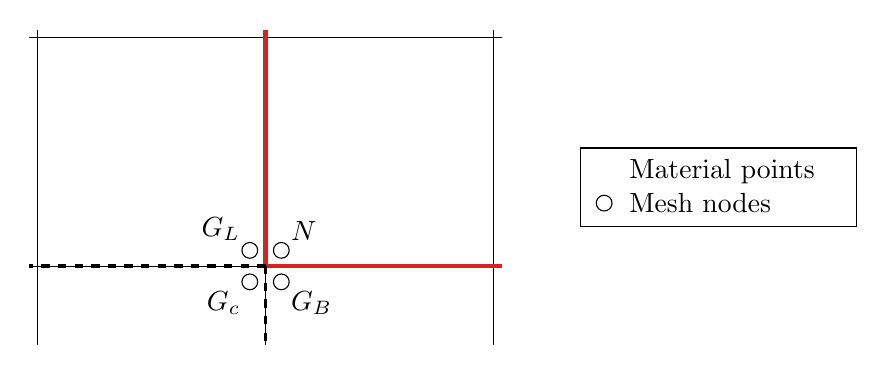
\begin{tikzpicture}
  \draw[step=2.9,black,thin] (-3.,-1.) grid (3,3.);
  \draw[ultra thick,Red] (0,3.) -- (0,0) -- (3.,0);
  % \draw[very thick,white] (0,0)--(0,-1.);
  % \draw[very thick,white] (0,0)--(-3.,-0.);
  \draw[very thick,dashed] (0,0)--(0,-1.);
  \draw[very thick,dashed] (0,0)--(-3.,-0.);
  \fill[white] (-0.2,-0.2) circle (0.1) node [below left] {$G_c$};
  \fill[white] (0.2,-0.2) circle (0.1) node [below right] {$G_B$};
  \fill[white] (-0.2,0.2) circle (0.1) node [above left] {$G_L$};
  \fill[white] (0.2,0.2) circle (0.1) node [above right] {$N$};    
  \draw[black] (-0.2,-0.2) circle (0.1) node [below left] {$G_c$};
  \draw[black] (0.2,-0.2) circle (0.1) node [below right] {$G_B$};
  \draw[black] (-0.2,0.2) circle (0.1) node [above left] {$G_L$};
  \draw[black] (0.2,0.2) circle (0.1) node [above right] {$N$};    
  \cross{0.3}{1.5};\cross{1.}{0.75};\cross{2.}{0.5};\cross{1.}{2.};
  \cross{2.5}{1.75};
  \draw (4.0,0.5) rectangle (7.5,1.5);
  \fill[white] (4.3,0.8) circle (0.1) node [right,black] {\: \text{Mesh nodes}};
  \draw[black] (4.3,0.8) circle (0.1);
  \cross{4.3}{1.2};
  \node[right] at (4.3,1.2) {\: \text{Material points}};
\end{tikzpicture}
  \caption{Corner ghost nodes in a two-dimensional DGMPM mesh.}
  \label{fig:corner_ghost}
\end{figure}

The transverse Riemann solver requires the introduction of corner ghost nodes equivalent to finite volume corner cells \cite{Leveque}. Consider the two-dimensional case depicted in figure \ref{fig:corner_ghost} in which boundary edges are represented by red lines. First, boundary interfaces are extended to the corner cell (vertical and horizontal dashed lines). Second, an inverse Riemann problem is solved between the corner ghost node $G_c$ and one regular ghost node, say $G_B$, so that the stationary solution of the Riemann problem between those ghost nodes corresponds to the boundary condition holding on the vertical edge. Third, this procedure is repeated between the corner ghost node and the regular one $G_L$ in order to enforce the boundary condition holding on the bottom boundary between them. 



\subsection{DGMPM solution scheme}
Let us assume that the vector of specific conserved quantities $\bar{\Wcb}^n$ as well as the auxiliary vector $\Qcb^n$ are known at every material points that discretize a continuum body $\Omega$ in a grid made of $N_{n}$ nodes at a given time $t^n$. We can now derive the computational steps to obtain the DGMPM solution for cases involving the auxiliary vector, the others are only particular cases of the precedure developed bellow.%, which requires to (i) solve the hyperbolic system \eqref{} in $\Omega$ with associated boundary conditions and (ii) update the vector $\bar{\Qcb}^n$ on material points.

The scheme has been established with a total Lagrangian formulation therefore, the weak form \eqref{eq:DGMPM_discrete_weak} is written on the reference configuration. Hence, the lumped mass matrix $M^L_i$ and the \textit{pseudo-stiffness} matrices $K^\alpha_{ij}$ are computed once and for all at the beginning of the calculation. Then, the procedure follows these steps:
\begin{itemize}
\item[] $\bar{\Wcb}, \:\Qcb$ known at material points
\item[(a)] Convective phase: the discrete equation \eqref{eq:DGMPM_discrete} and Riemann problems at cells interfaces \eqref{eq:RP_quasilinear} require a projection of fields onto the grid:
  \begin{equation}
    \label{eq:DGMPM_points2nodes}
    M^L_i \bar{\Wcb}^i = \sum_{p=1}^{N_p} S_{ip} m_p \bar{\Wcb}^p \qquad \text{and} \qquad M^L_i \vect{\Qc}^i = \sum_{p=1}^{N_p} S_{ip} m_p \vect{\Qc}^p 
  \end{equation}
  to be solved for each $\bar{\Wcb}^i$ and $\vect{\Qc}^i$ respectively. The projection of fields from particles to nodes hence follows the weighted least squares interpolation used in FLIP. 
%\item[(b)] Compute time step: in the general case the tangent modulus depends on the deformation gradient as well as the waves speeds. It is therefore needed to compute the time step so that the fastest wave can at most cross the smallest cell of the mesh according to Courant condition.
\item[(b)] The specific flux vectors $\bar{\Fcb}^i_{\alpha}$ involved in the equations are computed from $\vect{\Qc}^i$ knowing $\rho_0$, thus avoiding the computation of constitutive equations.
\item[(c)] Enforce boundary conditions on the ghost nodes of mesh.
\item[(d)] Computation of interface fluxes: 
  \begin{itemize}
  \item[1-] Build the state vectors $\vect{\Qc}_{X_N^{\pm}}$ based on $\vect{\Qc}^{i,n}$ where $i$ denotes the nodes belonging to the face on both sides of an interface.
  \item[2-] Compute the stationary solution $\Qcb^*$ by means of the approximate-state Riemann solver.
  \item[3-] Calculate the corresponding normal flux $\Fcb_N \(\Qcb^*\)$ by either using the DCU or the CTU approach.
  \end{itemize} 
\item[(e)] Advance solution in time by solving the discrete equation \eqref{eq:DGMPM_discrete} at each node.
\item[(f)] Back-mapping: as motivated at the end of the previous secttion, the nodal updated solution is projected to material points with the classical interpolation as in PIC:
  \begin{equation}
    \bar{\Wcb}^{n+1}_p = \sum_{i=1}^{N} S_{ip}\bar{\Wcb}^{i,n+1}
  \end{equation}
\item[(g)] Material point kinematics and constitutive model: The new solution $\bar{\Wcb}^{p,n+1}$ allows to increment the deformation $\vect{\varphi}(\vect{X},t)$ and to update stress components which will be used in the auxiliary vector for the next time step, through hyperelastic constitutive equations:
  \begin{align}
    & \vect{\varphi}^{p,n+1}_p = \vect{X}^p + \Delta t \vect{v}^{p,n+1} \\
    & \tens{\Pi}^{p,n+1} =  \drond{\Psi}{\tens{F}}(\tens{F}^{p,n+1})
  \end{align}
  The grid may then be discarded and reconstructed and especially by means of adaptive algorithms applied in the reference configuration, in order to improve wave front tracking in the current one.
\end{itemize}

Let's now recall or highlight significant differences between the DGMPM and the original MPM schemes. 
% Ouai ?
First, while the DGMPM uses a classical interpolation to mapping back the updated solution to material points (step f), FLIP method and MPM require an additional time integration on material points. 
% ok
Furthermore, the use of conservation laws \eqref{eq:conservative_form} instead of the momentum equation in the weak form implies that both velocity and gradients are solved at nodes making this new approach close to finite volume methods. 
% ok
Finally, the deformation gradient is no longer calculated with shape functions gradients so that the task of choosing between USF and USL algorithms vanishes. In that sense the DGMPM scheme is simpler though additional cost is linked to Riemann solutions. Fortunately, the use of discontinuous Galerkin approximation makes this numerical method highly parallelizable \cite{Cockburn}. The numerical scheme derived above is analyzed in terms of staiblity and convergence in the next secion.


%%% Local Variables: 
%%% mode: latex
%%% TeX-master: "../mainManuscript"
%%% End:
